\section{Security assessment}

what did we do?

    We conducted a security assessment of the system by:
    First identifying our assets, sources of threats and construct risk scenarios.
    Secondly we used the information from identifying to create a Risk analysis, we used placed the threats in a risk matrix and discussed solutions for the different 
    Thirdly we penetration tested the system by using two vulnerability scanners OWASP ZAP and Metasploit WMAP, targeting our .

    Try to resolve some of the vulnerabilities identified

why did we do it?

    to increase our awareness about the security of our system
    hands on experience with vulnerability scanners

what did we learn?

    Security is a vast topic and we have to be aware of it.
    We have to be aware of the different types of threats and think about how to mitigate them.


\subsection{What did we do}
1. Risk identification

    We identified risk factors in the following areas:
    SQL Injection, Broken access control(logging, monitoring) and vulnerable and outdated components.


2. Risk analysis

Insert risk matrix here.
\begin{wrapfigure}{l}{0.25\textwidth}
    \centering
    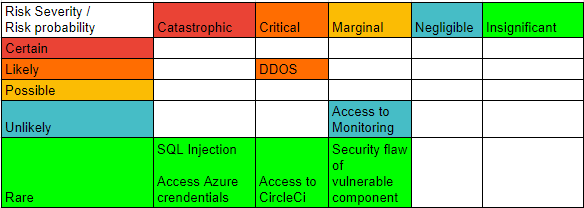
\includegraphics[width=0.25\textwidth]{RiskAssessmentMatrix.png}
\end{wrapfigure}

Insert key risk scenarios, maybe some we handled and some we did not.

3. penetration testing

    We used OWASP ZAP and Metasploit WMAP to test our system.
        vulnerability scanners
            OWASP ZAP
            Metasploit WMAP
    insert findings here.

    
4. which vulnerabilities did we resolve reflecitions

    
5. reflection / lessons learned?


I do not feel confident in saying the system is safe, I think the security aspect of a system would could be a course by it self.
But it was a good learning experience and using the vulnerability scanners and thinking about risk was valuable.

